%-----------------------------------------------
% Template para criação de relatórios de DAPI trabalho 3
% jlopes AT fe.up.pt,  Tue Dec 11 09:44:07 2007
%-----------------------------------------------

\documentclass[twocolumn,twoside,10pt,a4paper]{article}

%% packages
\usepackage[portuges]{babel}    % português
\usepackage{graphicx}           % images .png or .pdf w/ pdflatex OR .eps w/ latex
\usepackage[T1]{fontenc}
\usepackage{lmodern}            % fonts
\usepackage[utf8]{inputenc}     % 8 bits 
\usepackage{indentfirst}        % more on tables
\usepackage{lastpage}           % to have lastpage in headers
\usepackage{url}                % URLs
%\usepackage[pagebackref]{hyperref} %hyper-refs and back refs

% page layout
\RequirePackage[outer=20mm,inner=30mm,vmargin=20mm,includehead,includefoot,headheight=15pt]{geometry}

%% space between columns
\columnsep 12mm

%% headers & footers
\usepackage{fancyhdr}
\pagestyle{fancy}
\fancyhead{}            % clear all fields
\fancyhead[LE,RO]{\emph{MusicStats}}
\fancyhead[RE,LO]{}
\fancyfoot{}            % clear all fields
\fancyfoot[C]{\textit{\thepage\ de \pageref{LastPage}}}
\fancyfoot[LE,RO]{\textit{Grupo 9, \today}}
\renewcommand{\headrulewidth}{0pt}
\renewcommand{\footrulewidth}{0pt}
%\thispagestyle{plain}   % not in the 1st page
%% alternatively fancyplain could be used

% avoid widows and orphans
\clubpenalty=300
\widowpenalty=300

\title{MusicStats}

\author{Luís Dias\\Faculdade de Engenharia da Universidade do Porto\\080509094
\and
Luís Gomes\\Faculdade de Engenharia da Universidade do Porto\\080509169
}

\begin{document}

\maketitle

\begin{abstract}
O MusicStats consiste na concatenação da informação de dois datasets diferentes, o Last.fm e o MusixMatch.
Assim, através do cruzamento destes dois tipos de informação, criámos um novo dataset. Indexando os dados mais importantes, tornando assim a pesquisa menos morosa, conseguimos oferecer aos utilizadores as mais variadas informações acerca das músicas, tais como, quais as palavras mais usadas nas letras das músicas ou quais os temas de canções mais vendidas.
\end{abstract}

\section{Introdução}

Qual a banda de música que não gostaria de saber, à priori, que hipóteses tem da sua música nova de ser ouvida? Ou de todas as músicas existentes, quais os temas de canções que mais vende? Foi dessa necessidade que nasceu o MusicStats. No fim deste trabalho, pretende-se ter um dataset construído por nós, que servirá para auxiliar a análise musical actual. A partir daí, e com a informação presente, a imaginação é o limite, e será possível conjugar todos os dados das mais ínfimas formas. Saber qual o tipo de música mais usado, qual o tema de música tem mais influência nas músicas, quais as palavras mais usadas ou qual o tema preferido por cada banda aquando da criação das músicas. Para isso, criámos um dataset, que reusulta da concatenação entre o dataset da plataforma online, Last.fm, e o MusixMatch. Se no primeiro existe toda a informaçao de todas as músicas de um determinado artista, o segundo contempla todas as palavras pertencentes a uma letra de uma música. Assim sendo, o novo dataset por nós criado, para além das informações da música, contém todas as palavras presentes na sua letra.

Para realizar este trabalho foram consultadas variadas referências
bibliográficas relevantes, tais como
\begin{itemize}
\item \url{http://labrosa.ee.columbia.edu/millionsong/lastfm} Plataforma que contém toda a informação relevante do dataset do Last.FM
\item \url{http://www.lastfm.com.br/api} Plataforma que contém toda a informação relevante da API do Last.FM
\item \url{http://labrosa.ee.columbia.edu/millionsong/musixmatch} Plataforma que contém toda a informação relevante do dataset do MusixMatch
\item \url{https://developer.musixmatch.com/documentation} Plataforma que contém toda a informação relevante da API do MusixMatch
\end{itemize}

\section{Ferramenta a usar}\label{sec:ferramenta}

Para este trabalho, escolhemos a ferramenta \textit{open-source} Lucene. Com ela, podemos indexar o conjunto de dados que prentedemos, aumentando assim a velocidade das consultas. Para além disso, é uma ferramente com imensa documentação online, o que permite, também, uma rápida e fácil aprendizagem dos processos internos da ferramenta.

\section{Geraçao dos Índices}\label{sec:indices}

Como pretendemos dar resposta às interrogações dos utilizadores, teríamos obrigatoriamente que gerar alguns índices para aumentar a rapidez de resposta. Mas não faria sentido indexarmos todos os campos do dataset. Em primeiro lugar, porque seria um processo bastante moroso, em segundo lugar, porque não faria sentido indexar, por exemplo, campos relativos ao ID da música, pois não iria haver utilizadores a fazer interrogações por esse campo. Assim, estimámos quais os campos de pesquisa que mais vezes vão ser utilizados, e foram esses os escolhidos para a indexação. Como tal, indexámos os campo \textit{lyrics}, que tem todas as palavras da letra da música, \textit{artist}, que tem o nome do intérprete dessa música. Para isso, e tal como referido na secção anterior, utilizámos a biblioteca Lucene, que contempla funções de criação e gestão de índices, assim como auxiliares de pesquisa de informação.


\section{Demonstração do processo de interrogação}\label{sec:demonstração}



Como referido anteriomente, após o dataset estar devidamente construido, a sua consulta deve responder a uma variedade de perguntas, entre as quais podemos destacar:

\begin{itemize}
	\item Quais as palavras mais usadas em todas as canções;
	\item Qual o género de músicas mais usado;
	\item Qual o tema mais utilizado na composição de músicas;
	\item Qual a Banda que mais músicas tem sobre determinado tema;
	\item Quais as músicas que falam sobre determinado tema.
\end{itemize}

\begin{figure}[ht]
\centerline{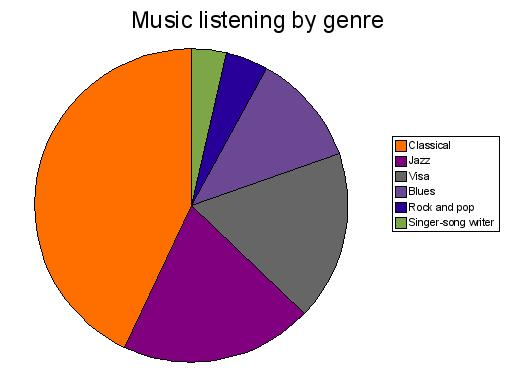
\includegraphics[scale=.36]{statistics.jpg}}
\caption{{\it Há géneros que são mais ouvidos que outros, mas terá isso alguma ligação com o tema?}}  
\label{fig:generos}
\end{figure}

\section{Conclusões}\label{sec:conclude}

Este sistema servirá para o correcto estudo e análise dos temas utilizados pelos compositores no acto de criação das próprias músicas. Nos tempos que correm, deve cada vez mais ser prestada a devida atenção ao meio envolvente, ao sucesso alheiro. Esta aplicação vem, precisamente, ao encontro dessa necessidade na medida em que estuda todos os elementos existentes no mercado, fazendo uma espécie de análise de êxito ou de fracasso. Analisa todas as canções para sabermos o que é mais utilizado, para, ou serem seguidas as mesmas directrizes, numa tentativa de sucesso seguro, ou tentar criar algo novo e inovador.

\begin{thebibliography}{4}  
\bibitem{MDSLast} Million Song Database. The Last.fm Dataset,URL: \textbf{http://labrosa.ee.columbia.edu/
millionsong/lastfm}, Outubro 2012.
\bibitem{Lastfm} Last.fm. API - Last.fm,URL: \textbf{www.last.fm/api}, Outubro 2012.
\bibitem{MDSmxm} Million Song Database.  The musiXmatch Dataset,URL: \textbf{http://labrosa.ee.columbia.edu/
millionsong/musixmatch}, Outubro 2012.
\bibitem{mxm} MusiXmatch. Documentation,URL: \textbf{https://developer.musixmatch.com/
documentation}, Outubro 2012.
\end{thebibliography}
%%%%%%%%%%%%% end %%%%%%%%%%%%%%%%%%%%%%%%%%%%%%%


\end{document}
